\section{Event Topology and the Spherical Harmonics Analysis}
\label{sec:topology_and_harmonics}

We have developed a method based on a spherical harmonics
decomposition to discriminate the topologies of 0\nbb-decay
two-electron events and \B-neutrino single-electron events. The
identification of the Cherenkov photon clusters is challenging due to
the smearing of the characteristic ring pattern by multiple scattering
of the electrons and by the smallness of the Cherenkov signal
relative to the large amount of uniformly-distributed scintillation
light.  We find that performing the spherical harmonics analysis on
the smaller early PE sub-sample, which has a relatively high fraction
of Cherenkov PEs, can discriminate 0\nbb-decay signal events from
backgrounds, although a high rejection factor will require a slower
scintillator than in the model.

\subsection{Topology of 0\nbb-decay and \B~Events}
\label{subsec:topology}

With \Te as the active isotope, all background from \B~solar neutrinos
will have the single electron above Cherenkov threshold in the liquid
scintillator. Also, a large fraction of 0\nbb-decay signal events will
have both electrons above Cherenkov threshold.

In some cases only one Cherenkov cluster is produced in 0\nbb-decay
signal events. This happens either when the angle between the two
0\nbb-decay electrons is small and Cherenkov clusters overlap or when
the energy split between electrons is not balanced, causing one
electron to be below Cherenkov threshold.  Such signal events cannot
be separated from background based on the topology of the distribution
of Cherenkov photons on the detector surface.  However, the
directionality of the electron that is above Cherenkov threshold can
still be reconstructed. This directionality information may allow for
suppression of \B~events based on the position of the
sun~\cite{sun_direction_cut}.

For the purpose of illustrating the spherical harmonics analysis
concept, we first consider two distinct topologies: a) two electrons
produced back-to-back at an 180$^{\circ}$ angle;  and b) a single electron.
Figure~\ref{fig:ThreeTopologies_Display_NoMultScat} shows an idealized
simulation of these two topologies for a total electron energy of
2.53~MeV. In order to emphasize ring patterns formed by Cherenkov
photons, the electron multiple scattering process is turned off in this
idealized simulation and a photocathode QE of 30\% is used for both
Cherenkov and scintillation photons. Here the single-electron event
represents an idealized \B~event topology and the two-electron events
represent two special cases of an idealized 0\nbb-decay topology.


\begin{figure*}[h]
  \centering
%  \begin{tabular}{c c c}
  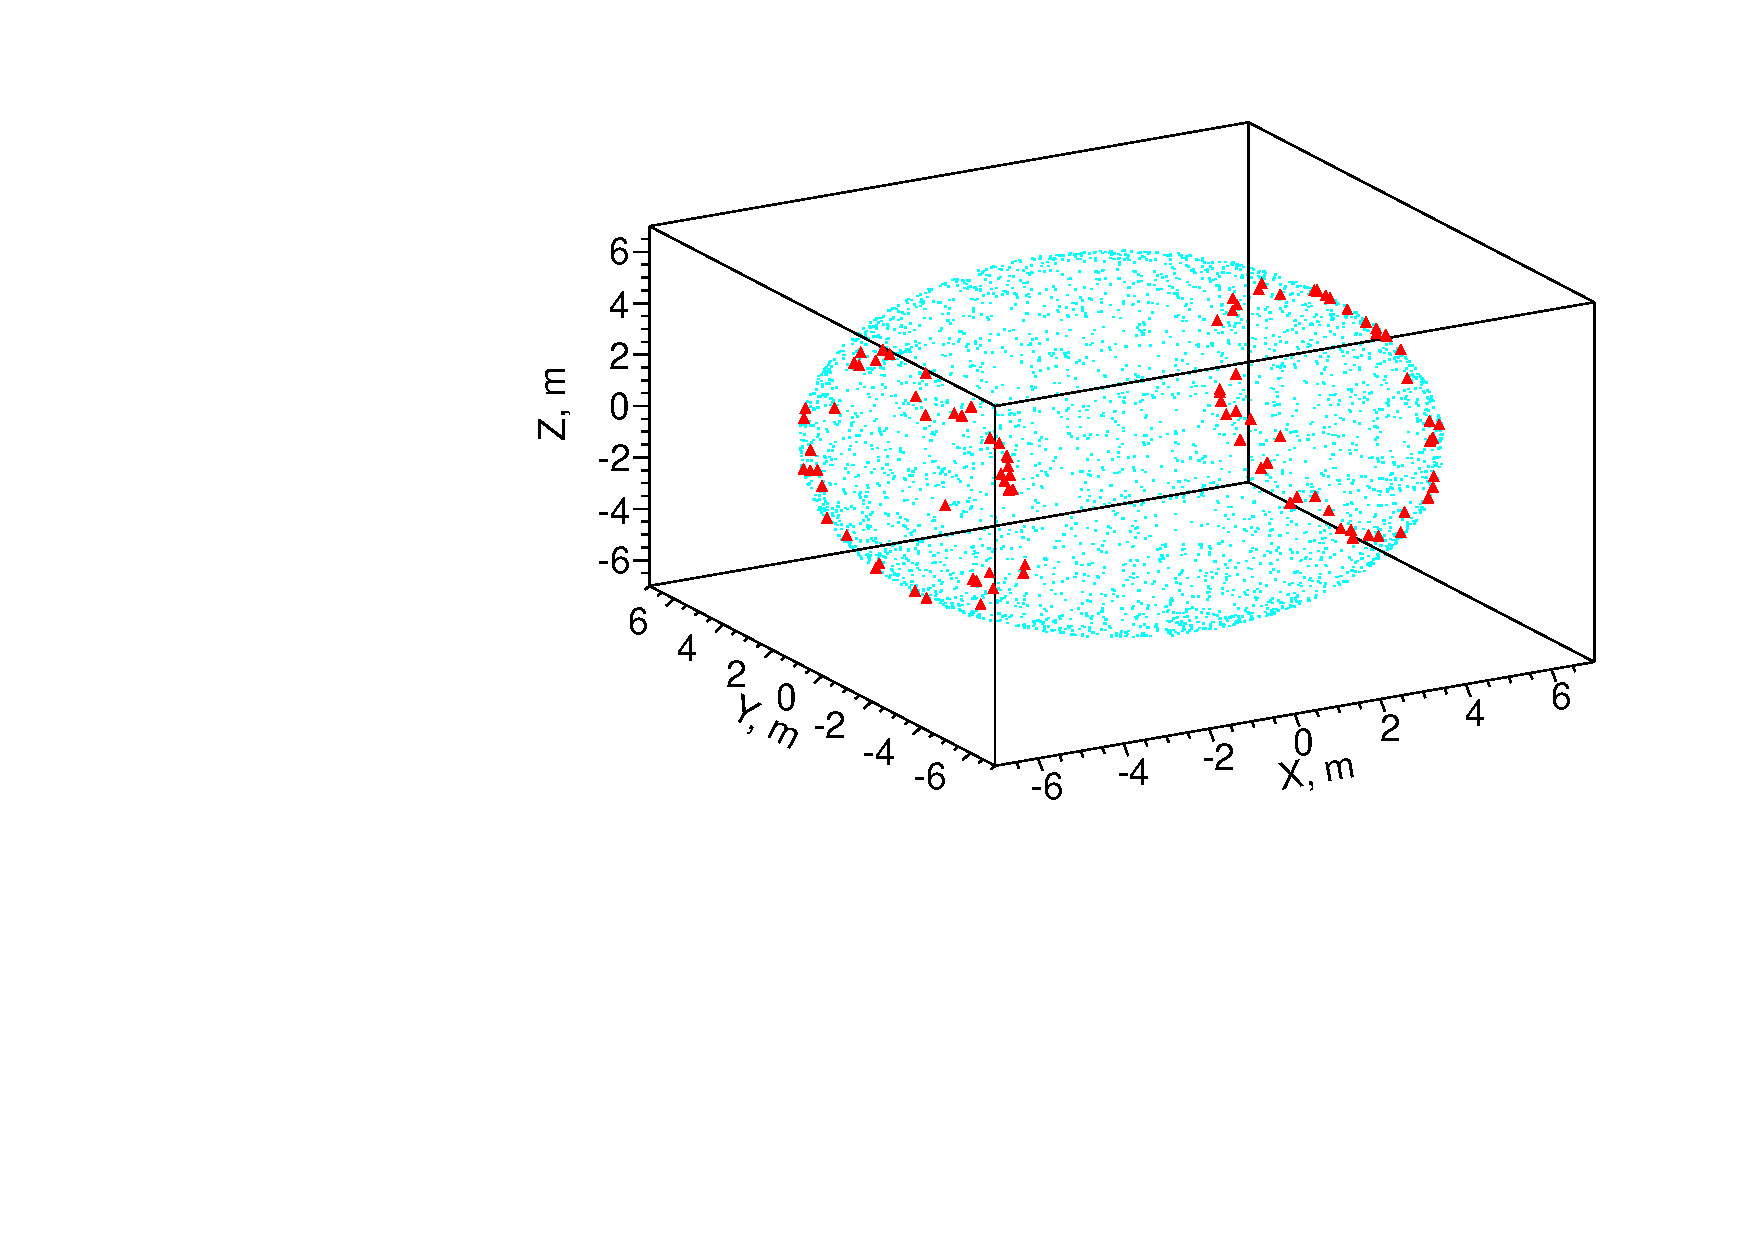
\includegraphics[width=0.45\textwidth]{hDisplay_topology180_NoMultScat.pdf}
%  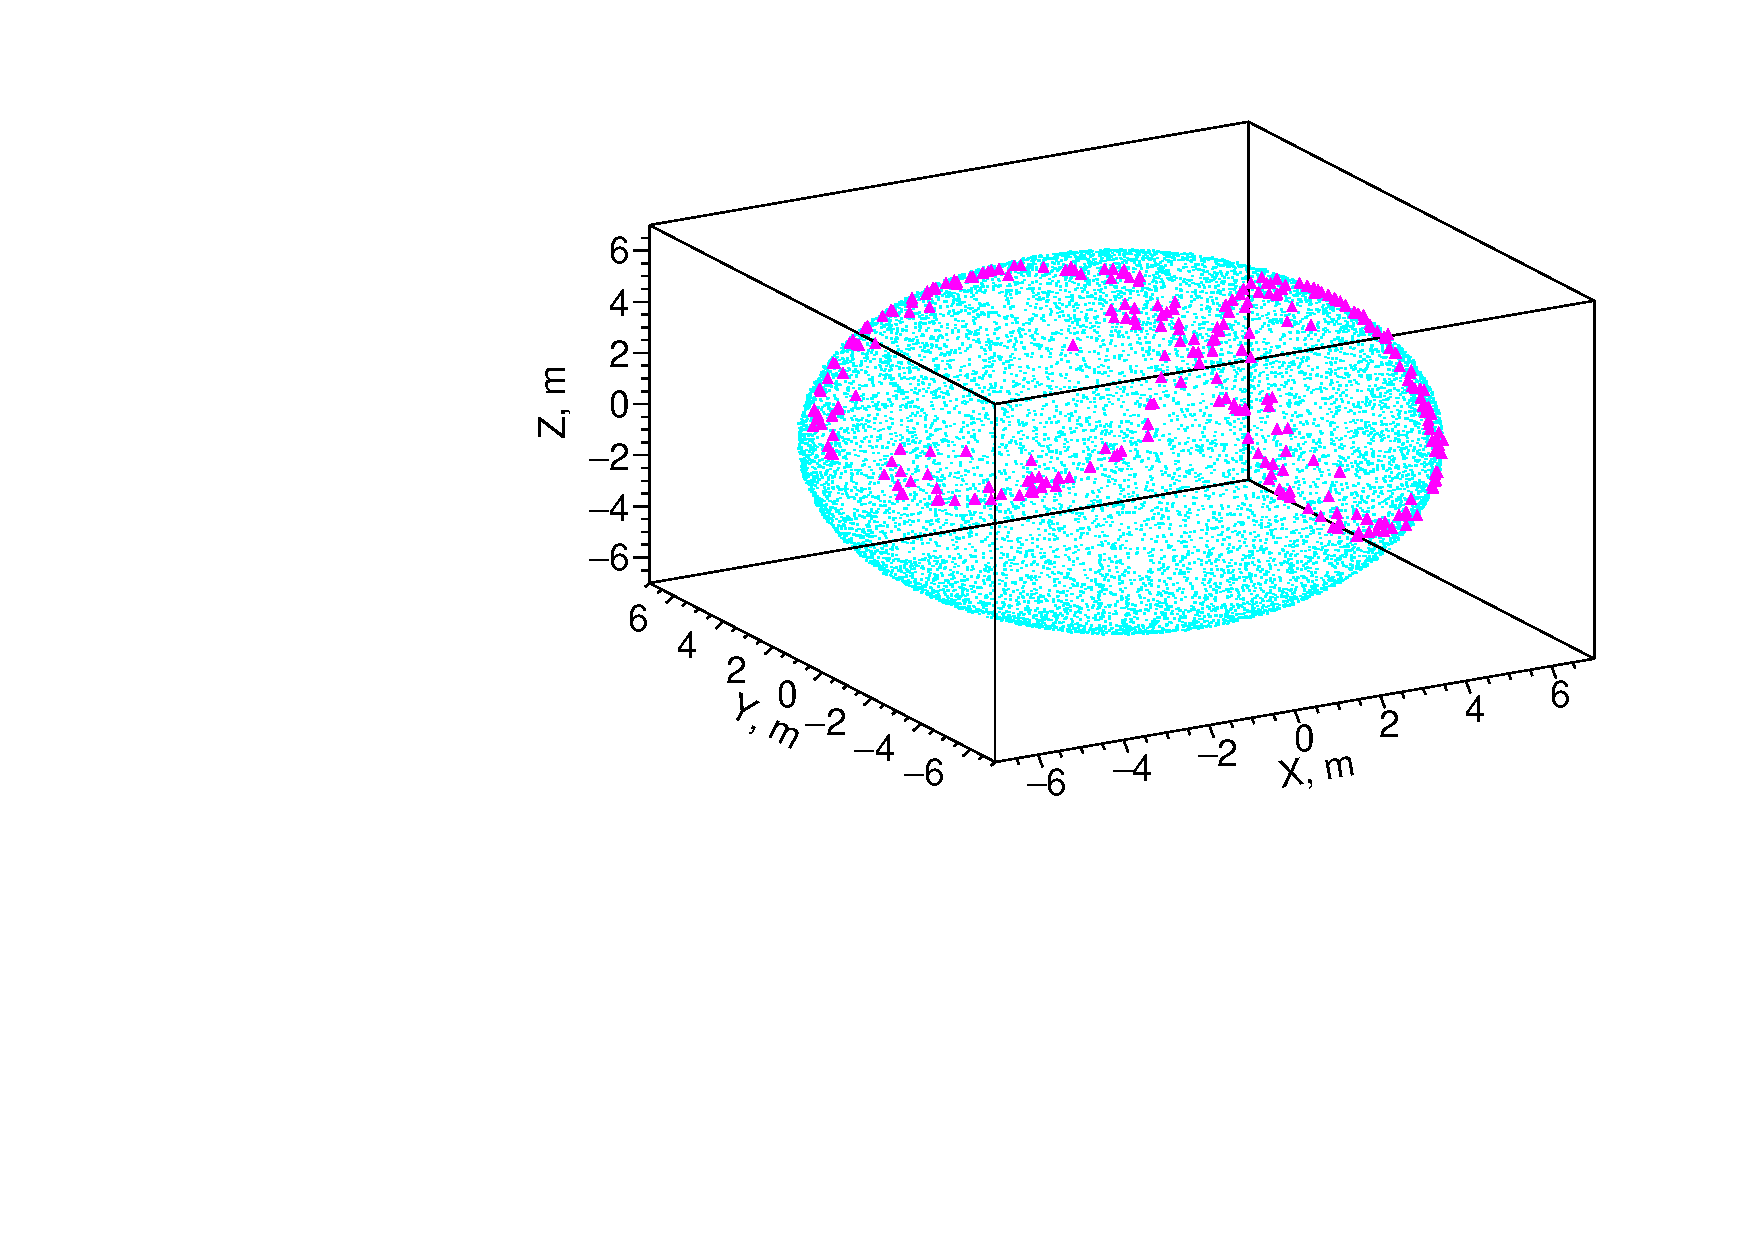
\includegraphics[width=0.33\textwidth]{hDisplay_topology90_NoMultScat.pdf}
  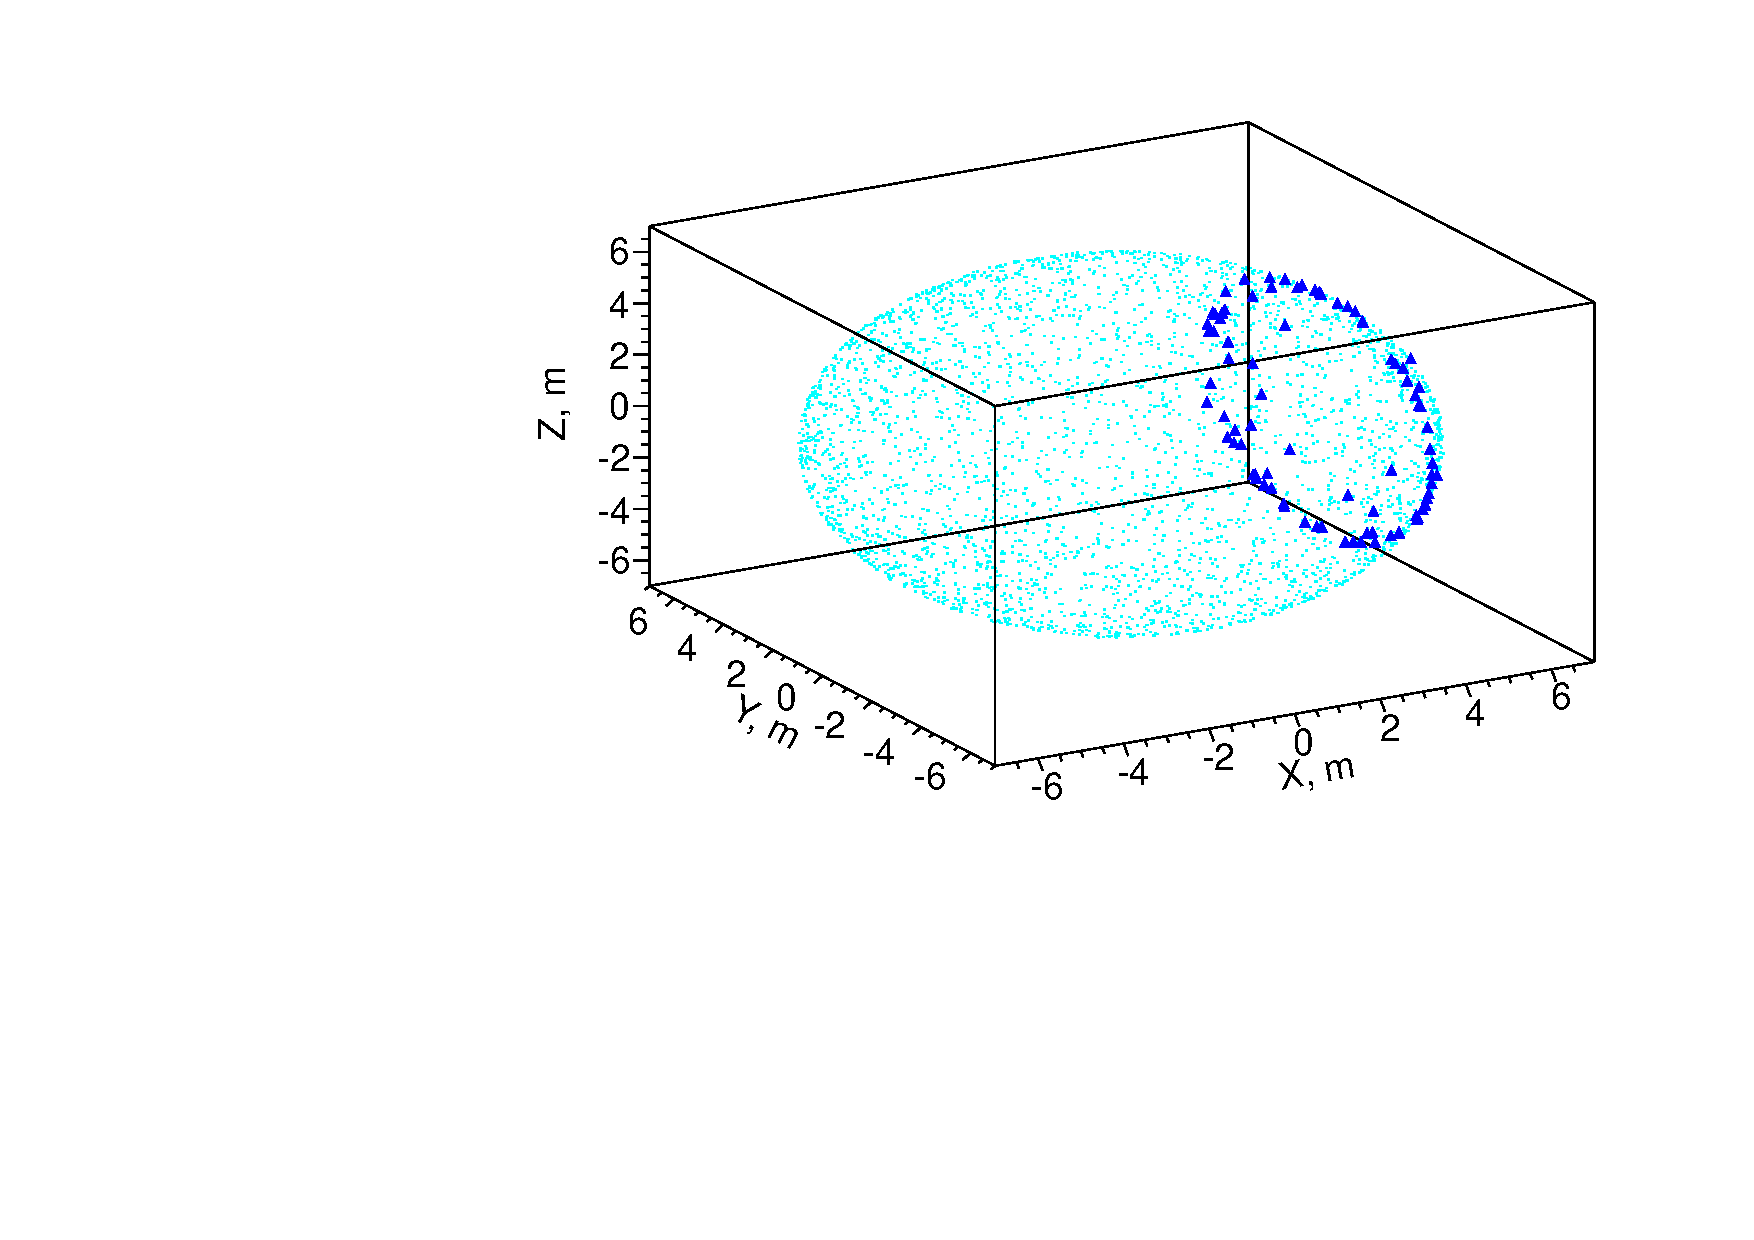
\includegraphics[width=0.45\textwidth]{hDisplay_1el_2p529MeV_NoMultScat.pdf}
%  \end{tabular}
  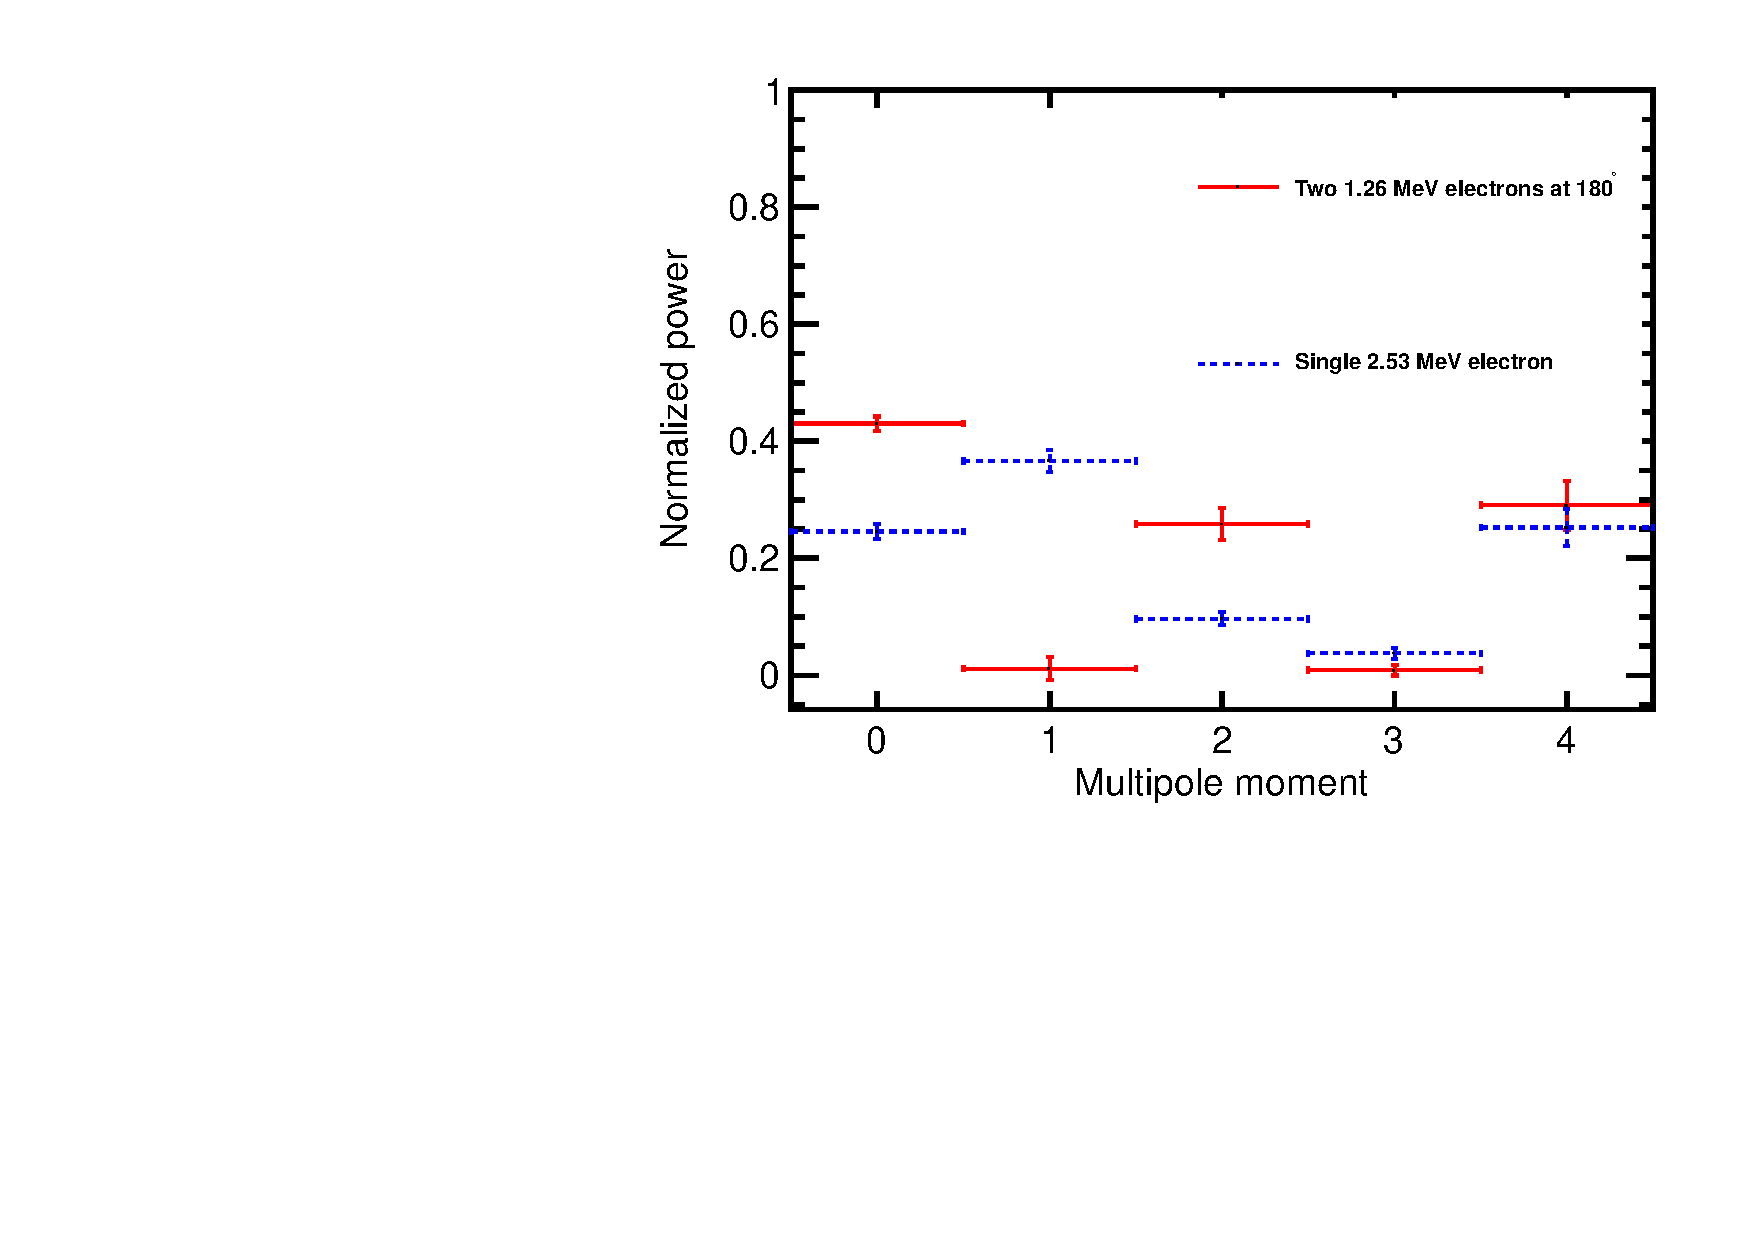
\includegraphics[width=0.9\textwidth]{hMultipleMoment_CHELight_VtxSmear0cm_VtxShiftX0cm_999p9ns_center_NoMultScat.pdf}
  \caption{\emph{Top panels:} Idealized event displays, with multiple
scattering turned off and at the center of the detector, of:
(\emph{top left}) a signal event with two 1.26~MeV back-to-back
electrons; and (\emph{top right })a \B-neutrino background event with
single 2.53~MeV electron. A 30\% QE is assumed for both Cherenkov
photons (triangles) and scintillation photons (dots).  
\emph{Bottom panel:} The normalized power spectrum $S_l$ for the
Cherenkov photons only, calculated event-by-event for the two
above topologies. The height of the rectangular boxes correspond to a 
63\% confidence level $(\pm 1 ~\sigma)$.}
  \label{fig:ThreeTopologies_Display_NoMultScat}
\end{figure*}


\subsection{Description of the Spherical Harmonics Analysis}

The central strategy of the spherical harmonics analysis is to
construct rotationally invariant variables that can be used to
separate different event topologies. To account for the fluctuation of
the number of PEs from event to event, we use a normalized power,
$S_l$, defined in Appendix A.

The bottom panel in Fig.~\ref{fig:ThreeTopologies_Display_NoMultScat}
compares the normalized power spectra for the two representative event
topologies in the idealized case of no multiple scattering and with a 30\%
quantum efficiency for both Cherenkov and scintillation
photons~\cite{QE}. The method gives a good separation between the
two event topologies.

However, at energies relevant to 0\nbb-decay the Cherenkov rings
become very fuzzy due to electron multiple scattering. In most cases,
$\sim$1~MeV electrons produce randomly shaped clusters of Cherenkov
photons around the direction of the electron track.  Examples of \Te~
0\nbb~and \B~events simulated with multiple scattering, but still at
the center of the detector, are shown in Fig.~\ref{fig:Te130_Display}.
\Te~ events are generated based on the phase factors described
in~\cite{Jenni}.  $^{8}$B events are implemented as
monochromatic electrons with the initial direction along the
$x$-axis. The default QEs of 12\% for Cherenkov light and 23\% for
scintillation light have been  applied. Figure~\ref{fig:Te130_Display} shows
early PEs that pass the 33.5~ns time cut. 
% fix the xxs

In this more realistic example, the uniformly distributed
scintillation light makes it difficult to visually distinguish
the event topology. The power spectra shown in the bottom panel of
Fig.~\ref{fig:Te130_Display}~ are different only at $l$=0 and
$l$=1. We use this difference to separate 0\nbb-decay
signal from \B~background events.

\begin{figure*}[hb]
  \centering
  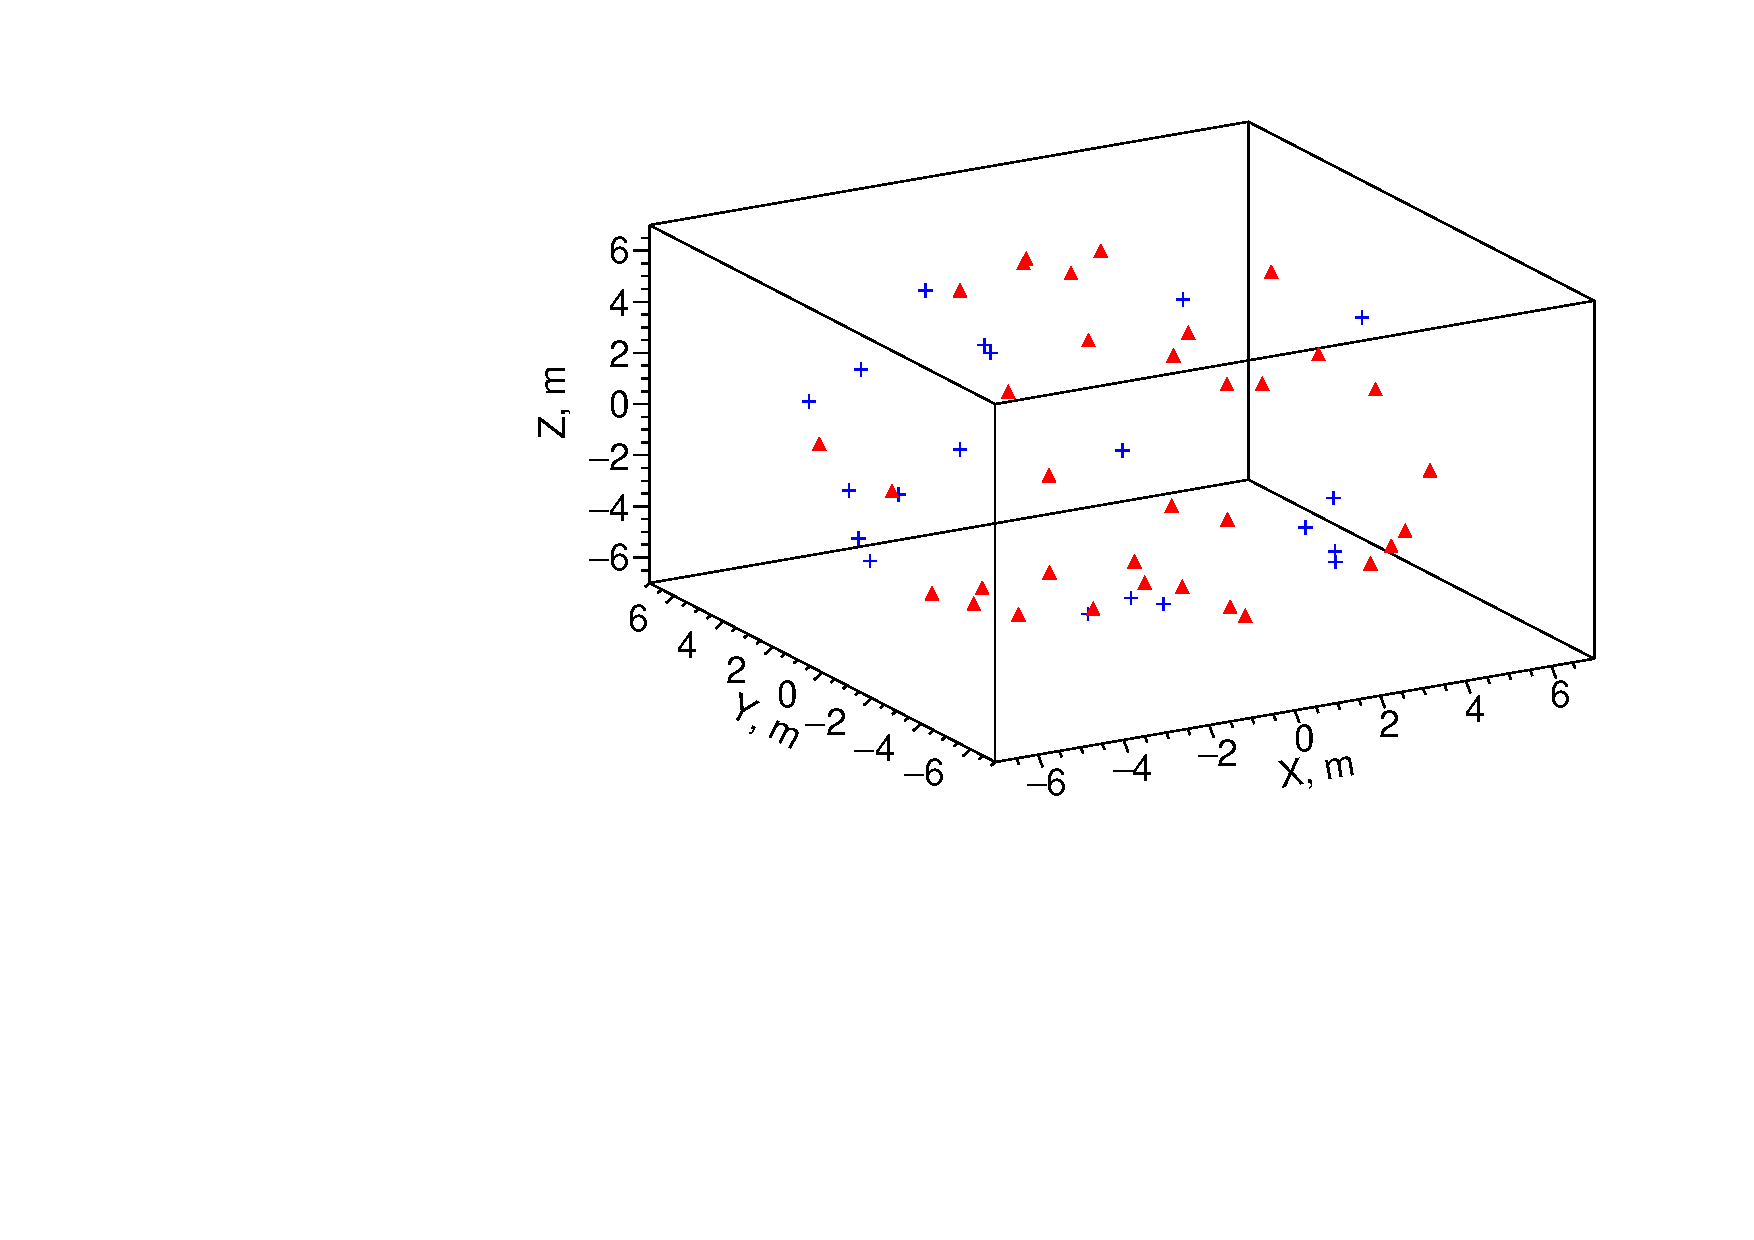
\includegraphics[width=0.42\textwidth]{hDisplay_Te130_evt124_e1257_e1270_cos-0908}
  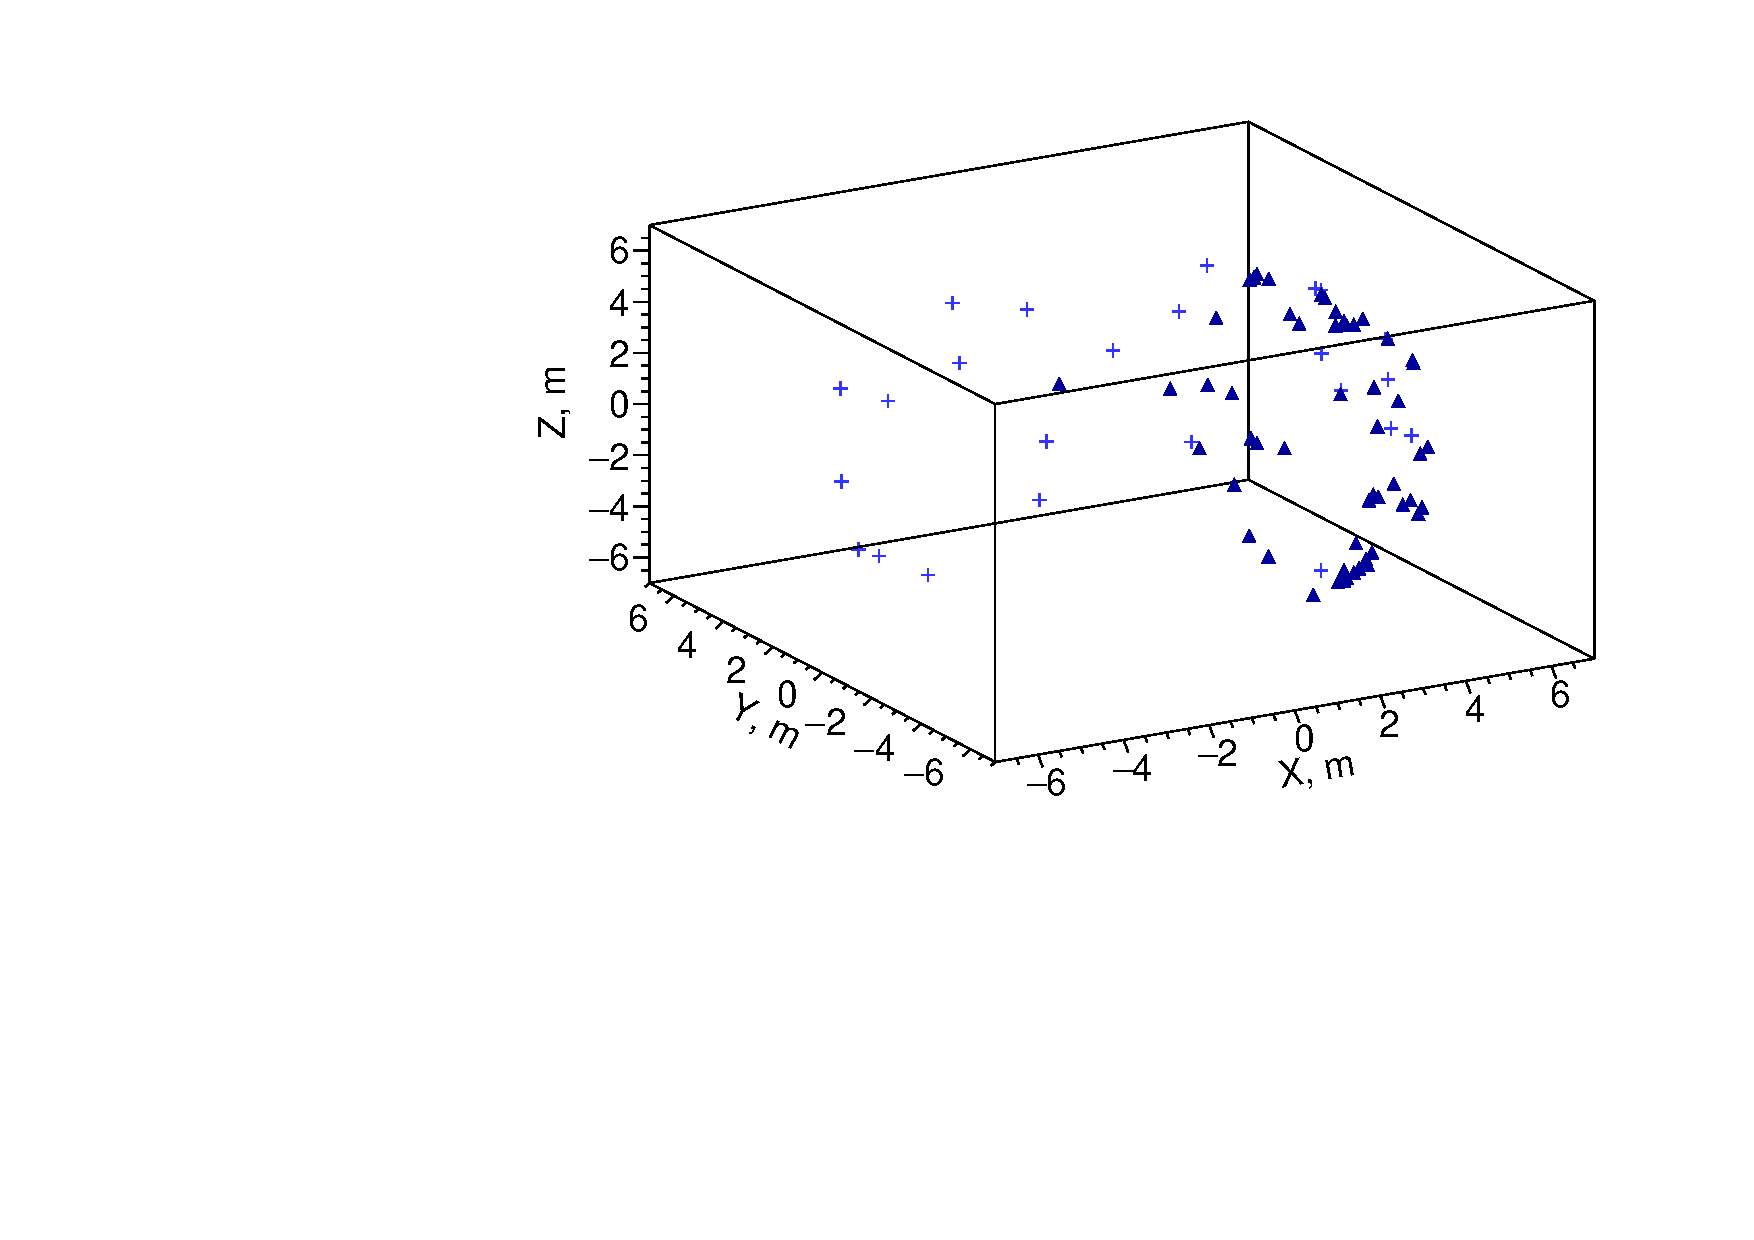
\includegraphics[width=0.42\textwidth]{hDisplay_1el_2p529MeV_33p5ns}
  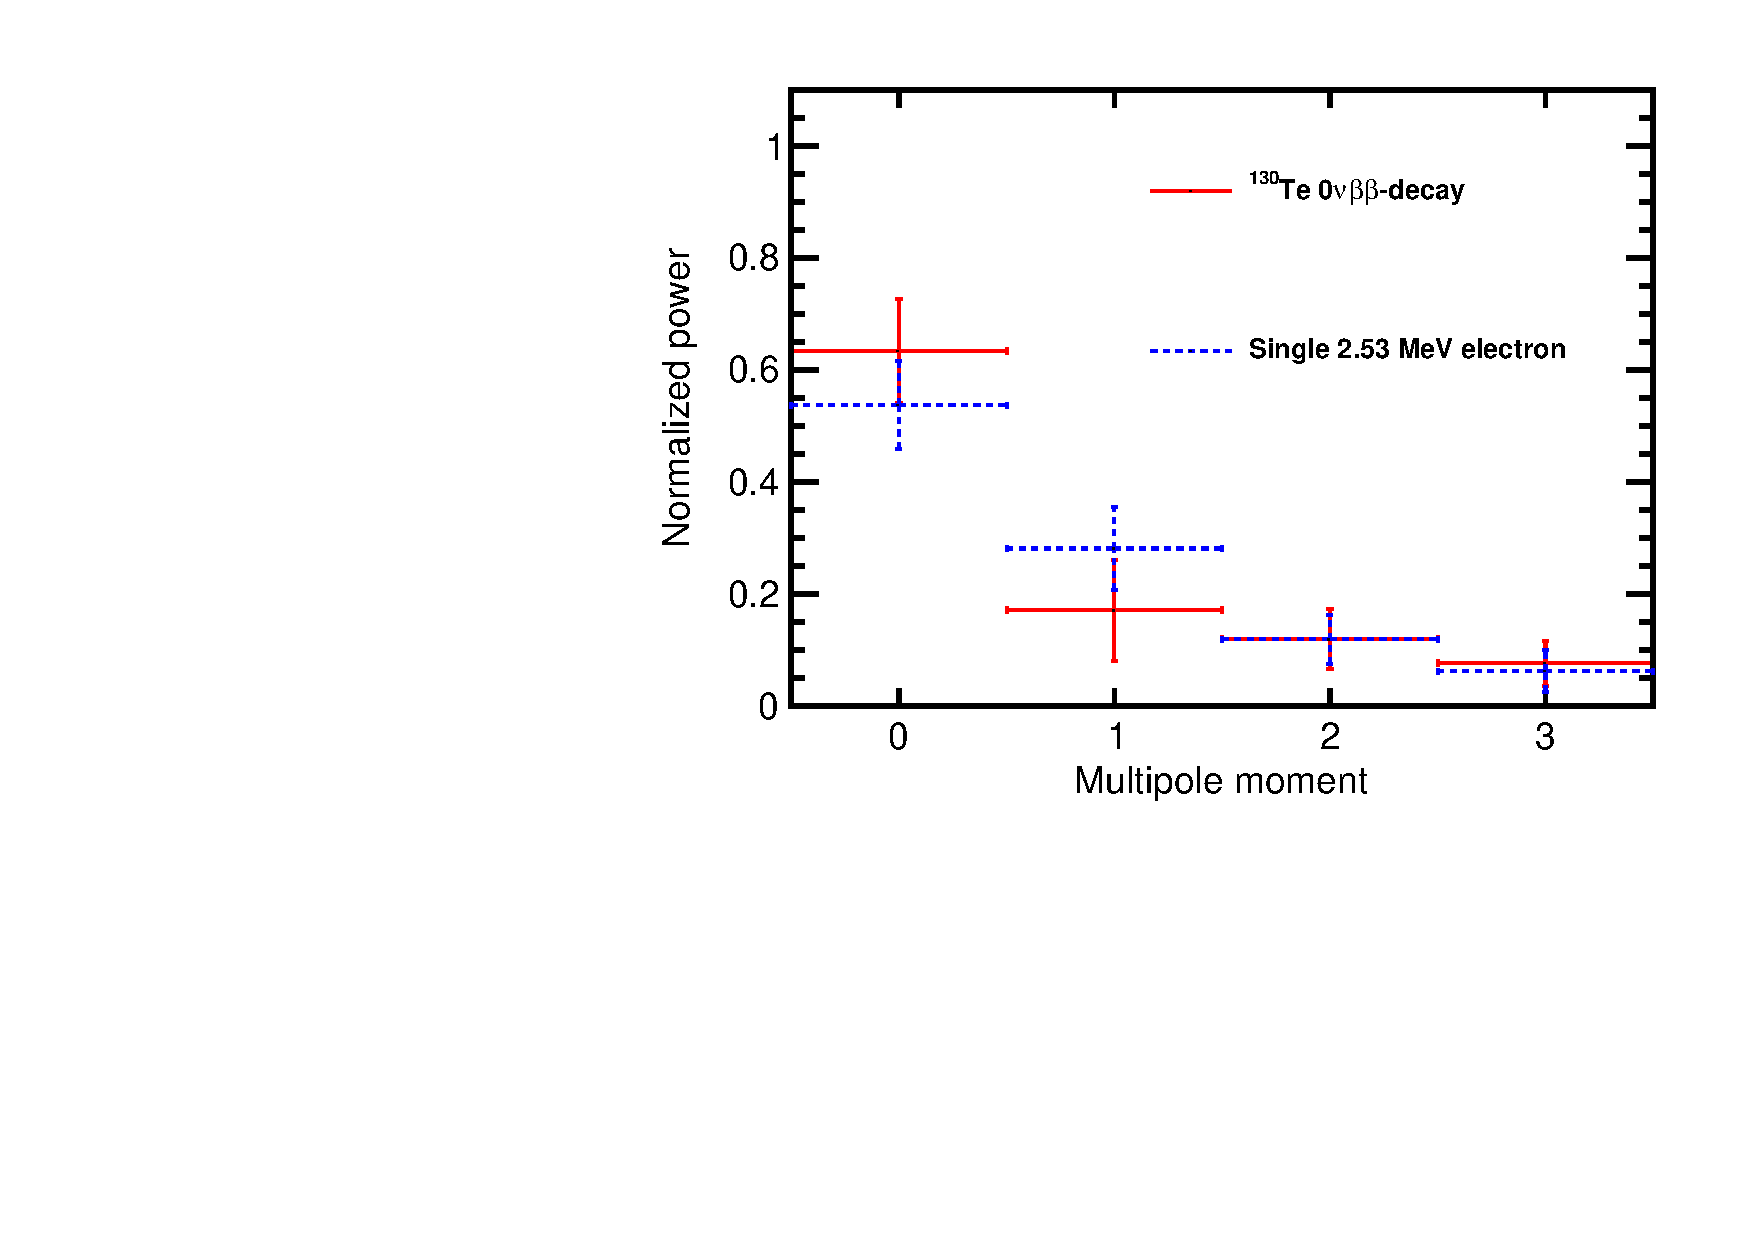
\includegraphics[width=0.8\textwidth]{hMultipleMomentSignal_allLight_VtxSmear0cm_VtxShiftX0cm_33p5ns_center.pdf} 
  \caption{\emph{Top panels:} Event displays with multiple scattering
and at the center of the detector for: (\emph{top left}) a signal
event with two 1.26~MeV back-to-back electrons; and (\emph{top right
})a \B-neutrino background event with a single 2.53~MeV electron. The
model QEs are assumed for both Cherenkov photons (triangles) and
scintillation photons (dots).  \emph{Bottom panel:} The normalized
power spectrum $S_l$ for the Cherenkov photons, calculated
event-by-event for 1000 events of each of the two above topologies. The
heights of the rectangular boxes correspond to a 63\% C.L.
$(\pm 1 ~\sigma)$.}
\label{fig:Te130_Display}
\end{figure*}

We find that 0\nbb~events become indistinguishable from single-track events when
the angle between the two electrons is small and two Cherenkov
clusters overlap. Event topologies of 0\nbb~and \B~events are also
very similar when only one electron from 0\nbb~ is above the Cherenkov
threshold. The spherical harmonics analysis is most efficient
for events with large angular separation between the two electrons and
when both electrons are above Cherenkov threshold~\cite{further_cuts}.



